\Chapter{Tervezés}

Bevezető szöveg...

\Section{Szerepkörök leírása}

A webalkalmazás kialakítása során hat különböző szerepkört határoztam meg, amelyek mindegyike különös felelősséggel és jogosultságokkal rendelkezik a platformon. Ezek a szerepkörök a következők:

\begin{enumerate}
\item Hallgató
\begin{itemize}
\item Szakdolgozat létrehozása, szerkesztése és mentése a rendszerben.
\item Az elkészült dolgozat benyújtása a rendszeren keresztül.
\item Visszajelzések és észrevételek megtekintése a dolgozatról a bírálók, témavezető vagy a bizottság részéről.
\item A bírálók és a bizottság értékeléseinek megtekintése.
\item A védés időpontjának és helyszínének megtekintése és kezelése.
\item A végső értékelés és jegy megtekintése.
\end{itemize}

\item Bíráló
\begin{itemize}
\item A dolgozat értékelése és visszajelzés küldése a hallgatónak.
\item A dolgozat nyomon követése és annak státuszának frissítése a rendszerben.
\item Az értékelőlap és a végső jegy rögzítése a rendszerben.
\end{itemize}

\item Záróvizsga jegyzője
\begin{itemize}
\item A záróvizsga időpontjának és helyszínének meghatározása és frissítése.
\item A záróvizsga résztvevőinek (hallgató, bírálók, bizottság) értesítése és meghívók kiküldése.
\item A záróvizsga jegyzőkönyvének vezetése és rögzítése a rendszerben.
\end{itemize}

\newpage
\item Záróvizsga bizottság elnöke
\begin{itemize}
\item A bizottság tagjainak kijelölése és módosítása.

\item A záróvizsga menetének és a kérdéseknek meghatározása.

\item A hallgató szakdolgozatának értékelése a bizottság véleménye alapján.

\item A végső értékelés rögzítése a rendszerben.
\end{itemize}

\item Témavezető

\begin{itemize}
\item A hallgatóval való kommunikáció és támogatás a szakdolgozat elkészítése során.

\item A hallgató dolgozatának nyomon követése és visszajelzések küldése.

\item A bírálók és a bizottság értékeléseinek megtekintése.

\item A végső értékelés és jegy rögzítése a rendszerben.


\end{itemize}

\item Adminisztrátor

\begin{itemize}

\item Az adminisztrátor a fentiek mindegyikével rendelkezik.

\end{itemize}

\end{enumerate}

\begin{figure}[h]
\centering
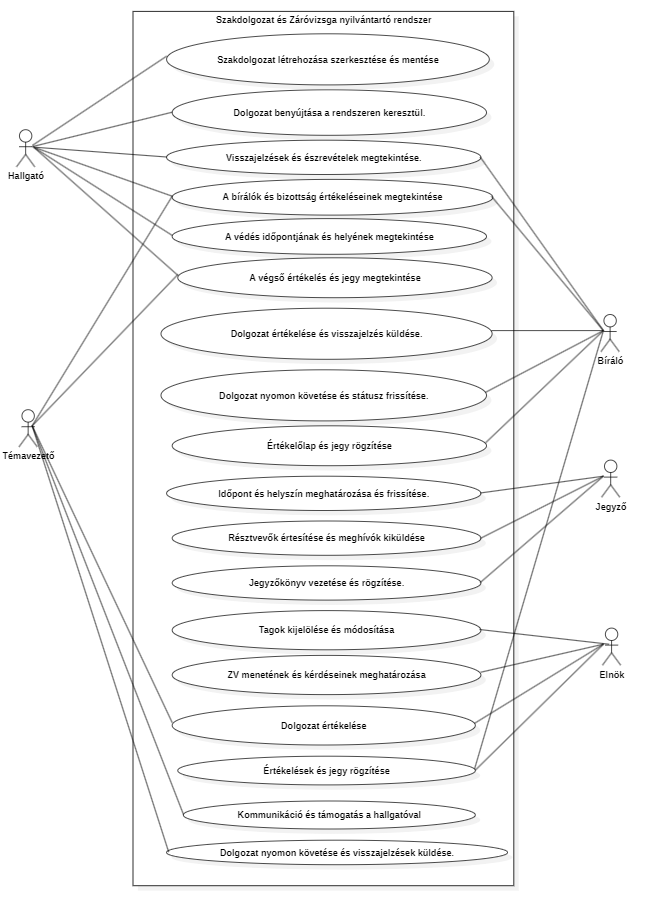
\includegraphics[scale=0.5]{images/Use_case_diagram.png}
\caption{Az alkalmazás use case diagramja}
\label{fig:usecase}
\end{figure}

\Section{Folyamatok ábrázolása}

Az alkalmazás tervezésekor több folyamatot is figyelembe kellett vennem, mint például a bírálati folyamat és a bírálat feltöltésének lépései. Ezeket a folyamatokat szekvenciadiagramon és folyamatábrán ábrázoltam.

\subsection{Bírálati folyamat}

\vspace{0.5cm}

\begin{enumerate}
\item \textbf{Adminisztrátor regisztrálja a hallgatót:}

Az adminisztrátor bejelentkezik az alkalmazásba és regisztrálja a hallgatót a rendszerbe.
A regisztráció során az adminisztrátor rögzíti a hallgató nevét, e-mail címét, jelszavát és egyéb szükséges információkat.

\item \textbf{Témavezető értesíti az adminisztrátort a bíráló elérhetőségéről:}

A témavezető értesíti az adminisztrátort arról, hogy mely bírálók érhetők el a szakdolgozat bírálásához. 

\item \textbf{Adminisztrátor regisztrálja a bírálót:}

Az adminisztrátor rögzíti a bíráló adatait az alkalmazásban, beleértve a nevet, e-mail címet, jelszót és egyéb szükséges információkat. A regisztráció után a bíráló jogosult lesz részt venni a bírálati folyamatban.

\item \textbf{Elnök felkéri a témavezetőt és a bírálót a bírálatra:}

Az elnök bejelentkezik az alkalmazásba és kiválasztja a szakdolgozatot, amelyre bírálatot kíván kérni. Az elnök elküldi a felkérést mind a témavezetőnek, mind a kiválasztott bírálónak a bírálat elvégzésére.

\item \textbf{Bíráló és témavezető elkészíti a bírálatot:}

Mind a bíráló, mind a témavezető bejelentkezik az alkalmazásba, ahol elérhetik a kijelölt szakdolgozatot. A bíráló és a témavezető részletesen értékeli a dolgozatot, és dokumentálja az észrevételeit, értékeléseit és esetleges javaslatait.

\item \textbf{Elnök kiküldi a bírálatot a hallgatónak:}

Az elnök bejelentkezik az alkalmazásba, ahol hozzáfér a bírálati eredményekhez.
Az elnök elküldi a bírálati eredményeket a hallgatónak, lehetővé téve számára azok megtekintését.
\end{enumerate}

\newpage

\begin{figure}[h]
\centering
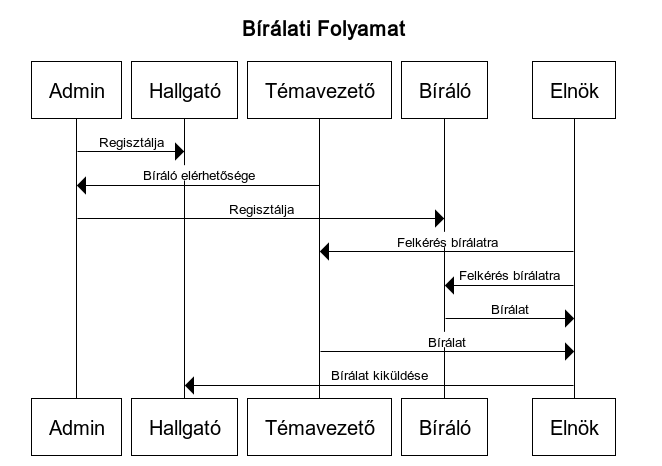
\includegraphics[scale=0.8]{images/Bírálati_folyamat.png}
\caption{Bírálati folyamat szekvenciadiagramja}
\label{fig:biralati_folyamat}
\end{figure}

\subsection{Bírálat feltöltésének lépései}

\begin{enumerate}

\item Bíráló belép a rendszerbe és listázza a felkéréseket:

A bíráló bejelentkezik az alkalmazásba a saját hitelesítő adataival.
Miután sikeresen bejelentkezett, a rendszer megjeleníti a bíráló számára elérhető felkéréseket listázó oldalt.
A felkérések listája tartalmazza az összes olyan feladatot vagy munkát, amelyekre a bírálót felkérték bírálat készítésére.

\item Bíráló kiválaszt egy felkérést a listából:

A bíráló kiválasztja a listából azt a felkérést, amelyre bírálatot szeretne készíteni.
A felkérés részletei megjelennek a bíráló számára, például a feladat neve, a beküldési határidő stb.

\item Bíráló elkezdi szerkeszteni a bírálatot:

A bíráló megnyitja a kiválasztott felkérést és elkezdi szerkeszteni a bírálatot.
A bíráló részletesen értékeli a feladatot vagy munkát, és dokumentálja az észrevételeit, pontozását vagy egyéb megjegyzéseit a bírálatban.

\item Bíráló beküldi a szerkesztett bírálatot:

Miután a bíráló elkészítette a bírálatot, beküldi azt a rendszerbe.

\item Ellenőrzés:

A rendszer ellenőrzi a beküldött bírálatot, hogy megfelel-e a formai követelményeknek.
Ha a bírálat formailag nem megfelelő:
A rendszer hibaüzenetet jelenít meg, és figyelmezteti a bírálót a hibákra.
A bíráló visszairányításra kerül a bírálat szerkesztéséhez, hogy kijavítsa a hibákat.
Ha a bírálat megfelelő formában van beküldve:
A rendszer értesítést küld a bírálónak a sikeres beküldésről.
A beküldött bírálat letöltődik a bíráló számítógépére az archiválás és további referenciák céljából.

\item A folyamat véget ér:

Miután a bíráló sikeresen beküldte és ellenőrizte a bírálatot, a folyamat befejeződik, és a bíráló visszatér az alkalmazás főoldalára vagy más tevékenységekhez.

\end{enumerate}

\begin{figure}[h]
\centering
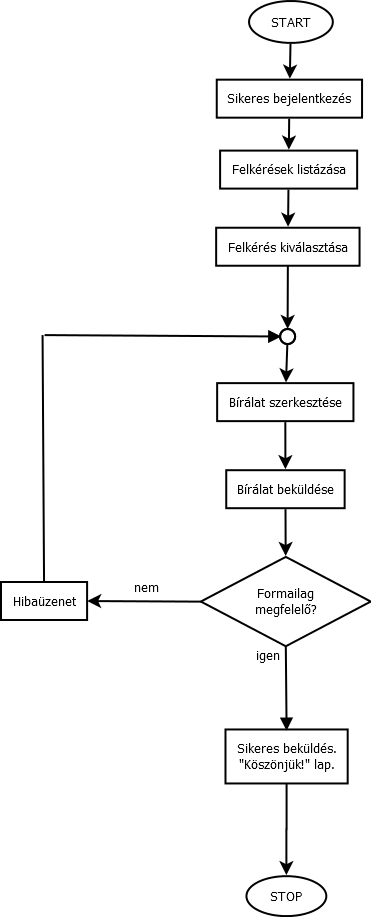
\includegraphics[scale=0.5]{images/Bírálat_feltöltése.png}
\caption{Bírálati feltöltéseinek lépései}
\label{fig:birala_feltoltese}
\end{figure}
